%
% Sample SBC book chapter
%
% This is a public-domain file.
%
% Charset: ISO8859-1 (latin-1) áéíóúç
%
\documentclass{SBCbookchapter}
\usepackage[utf8]{inputenc}
\usepackage[T1]{fontenc}
\usepackage[brazilian,english]{babel}
\usepackage{graphicx}

\author{Diego Fernando de Sousa Lima, Leonardo Augusto Gomes da Silva}
\title{Uma Introdução ao Go: A Linguagem Performática do Google}

\begin{document}
\maketitle

\begin{abstract}
This meta-paper describes the style to be used in articles and short
papers for SBC conferences. For papers in English, you should add just
an abstract and for the papers in Portuguese, we also ask for an
abstract in Portuguese (``resumo''). In both cases, abstracts should not
have more than 10~lines and must be in the first page of the paper.
\end{abstract}

\begin{resumo}
\begin{otherlanguage}{brazilian}
Este meta-artigo descreve o estilo a ser usado na confecção de artigos
e resumos de artigos para publicação nos anais das conferências
organizadas pela SBC.  solicitada a escrita de resumo e abstract apenas
para os artigos escritos em português. Artigos em inglês, deverão
possuir apenas abstract. Nos dois casos, o autor deve tomar cuidado para
que o resumo (e o abstract) não ultrapassem 10~linhas cada, sendo que
ambos devem estar na primeira página do artigo.
\end{otherlanguage}
\end{resumo}

\section{Introdução}
\subsection{Porque Go}
\subsection{Histórico}
\subsection{Go atualmente}

\section{Instalando e configurando o Go}
\subsection{Windows}
\subsection{Linux}
\subsection{Mac OS}

\section{Estrutura básica e sintaxe}
\subsection{Hello World}
\subsection{Variáveis}
\subsection{Estruturas de seleção}
\subsection{Exemplo 1}
\subsection{Exemplo 2}

\section{Coleções de dados}
\subsection{Arrays}
\subsection{Slices}
\subsection{Maps}
\subsection{Exemplo 1}
\subsection{Exemplo 2}

\section{Loops}

\section{Switch Case}

\section{Tipos estruturados de dados}
\subsection{Structs}
\subsection{Criando novos tipos}
\subsection{Interfaces}
\subsection{Duck typing}

\section{Funções}
\subsection{Funções básicas}
\subsection{Retorno definido}
\subsubsection{Defer}
\subsection{Funções de argumentos variáveis}
\subsection{Funções anônimas}
\subsection{Funções de primeira classe}
\subsection{Clojures}

\section{Tratamento de erros}

\section{Concorrência}
\subsection{Goroutines}
\subsection{Waitgroups}
\subsection{Channels}
\subsection{Controle de fluxo}
\subsubsection{Select}
\subsection{Timeouts}
\subsection{GOMAXPRO}

\section{Pacotes Go}
\subsection{Criando um pacote Go}
\subsection{Bibliotecas úteis}
\subsubsection{Time}
\subsubsection{Io/util e Os}
\subsection{Pacotes externos}

\section{Web com Go}
\subsection{O módulo  http/net}
\subsection{Frameworks Web Go}
\subsection{Beego}
\subsection{Construíndo uma API REST em Go}

\section{Extras}
\subsection{Integrando Go ao C}
\subsection{Bibliotecas de Machine Learning}



\begin{figure}[h!]
	\centerline{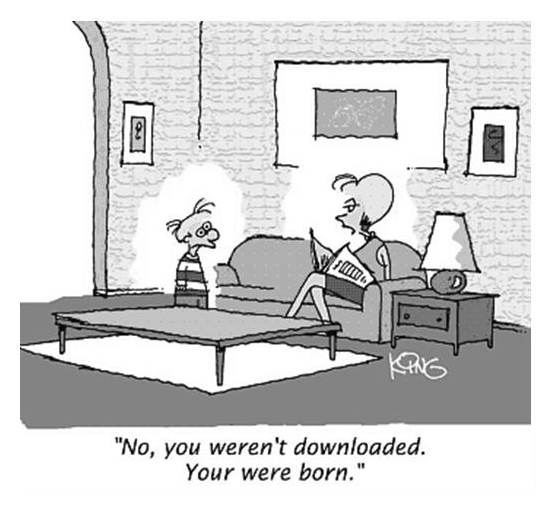
\includegraphics{fig1}}
	\caption{A typical figure}
	\label{figone}
\end{figure}



Figure and table references must be composed by the chapter number and
a sequence number beginning in one (see the examples of
Figure~\ref{figone}, Figure~\ref{figtwo} and Table~\ref{tabone}).

\begin{figure}[h!]
	\centerline{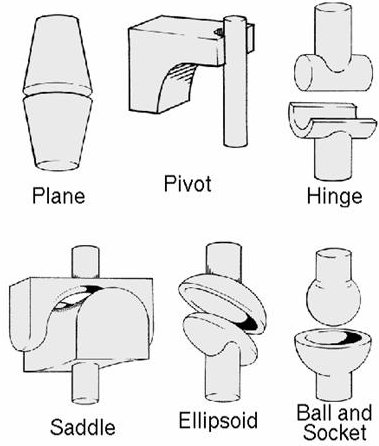
\includegraphics{fig2}}
	\caption{This figure is an example of a figure caption taking
		more than one line and justified considering margins
		mentioned in Section~\ref{sec:captionmargins}}
	\label{figtwo}
\end{figure}



\section{References}
Bibliographic references must be unambiguous and uniform.  We
recommend giving the author names references in brackets,
e.g.~[Knuth~1984], [Kernighan and Ritchie~1990]; or dates in
parentheses, e.g.~Knuth (1984), Sederberg and Zundel (1989,1990).

% you should really use BibTeX instead of this... :-)
\begin{thebibliography}{99}
\bibitem{bou91} Boulic, R. and Renault, O. (1991) ``3D Hierarchies for
  Animation'', In: New Trends in Animation and Visualization, Edited
  by Nadia Magnenat-Thalmann and Daniel Thalmann, John Wiley \& Sons
  ltd., England.

\bibitem{dye95} Dyer, S., Martin, J. and Zulauf, J. (1995) ``Motion
  Capture White Paper'',
  http://reality.sgi.com/employees/jam\_sb/mocap/MoCapWP\_v2.0.html,
  December.

\bibitem{hol95} Holton, M. and Alexander, S. (1995) ``Soft Cellular
  Modeling: A Technique for the Simulation of Non-rigid Materials'',
  Computer Graphics: Developments in Virtual Environments, R. A.
  Earnshaw and J. A. Vince, England, Academic Press Ltd., p.~449-460.

\bibitem{knu84} Knuth, D. E., The TeXbook, Addison Wesley, 1984.
\end{thebibliography}

\end{document}
